% This work is made available under the terms of the 
% Creative Commons Attribution-ShareAlike 4.0 license,
% http://creativecommons.org/licenses/by-sa/4.0/.

\documentclass[a4paper]{book}

\usepackage{wrapfig}
\usepackage{graphicx}
\usepackage{hyperref}
\usepackage{multirow}
\usepackage{scalefnt}
\usepackage{tikz}

% watermark -- for draft stage
\usepackage[firstpage]{draftwatermark}
\SetWatermarkLightness{0.9}
\SetWatermarkScale{5}

% Copyright (c) 2009 by the University of Waikato, Hamilton, NZ. 
% This work is made available under the terms of the 
% Creative Commons Attribution-ShareAlike 4.0 license,
% http://creativecommons.org/licenses/by-sa/4.0/.
%
% Version: $Revision: 6032 $

\newenvironment{tight_itemize}{
\begin{itemize}
  \setlength{\itemsep}{1pt}
  \setlength{\parskip}{0pt}
  \setlength{\parsep}{0pt}}{\end{itemize}
}

\newenvironment{tight_enumerate}{
\begin{enumerate}
  \setlength{\itemsep}{1pt}
  \setlength{\parskip}{0pt}
  \setlength{\parsep}{0pt}}{\end{enumerate}
}

% if you just need a simple heading
% Usage:
%   \heading{the text of the heading}
\newcommand{\heading}[1]{
  \vspace{0.3cm} \noindent \textbf{#1} \newline
}

\newcommand{\icon}[1]{\tikz[baseline=-3pt]\node[inner sep=0pt,outer sep=0pt]{\includegraphics[height=1.1em]{#1}};}


\title{
  \textbf{ADAMS} \\
  {\Large \textbf{A}dvanced \textbf{D}ata mining \textbf{A}nd \textbf{M}achine
  learning \textbf{S}ystem} \\
  {\Large Module: adams-spectral-3way-core} \\
  \vspace{1cm}
  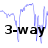
\includegraphics[width=2cm]{images/spectral-3way-core-module.png} \\
}
\author{
  Peter Reutemann
}

\setcounter{secnumdepth}{3}
\setcounter{tocdepth}{3}

\begin{document}

\begin{titlepage}
\maketitle

\thispagestyle{empty}
\center
\begin{table}[b]
	\begin{tabular}{c l l}
		\parbox[c][2cm]{2cm}{\copyright 2017-2018} &
		\parbox[c][2cm]{5cm}{
\includegraphics[width=5cm]{images/coat_of_arms.pdf}} \\
	\end{tabular}
	
\includegraphics[width=12cm]{images/cc.png} \\
\end{table}

\end{titlepage}

\tableofcontents
%\listoffigures
%\listoftables

%%%%%%%%%%%%%%%%%%%%%%%%%%%%%%%%%%%
\chapter{Flow}
The following transformers are available:
\begin{tight_itemize}
  \item \textit{ThreeWayDataFileReader} -- for reading data form disk in a
  specific format.
  \item \textit{ThreeWayDataFileWriter} -- for writing data to disk in a
  specific format.
  \item \textit{ThreeWayDataFilter} -- for applying a filter to the 3-way data.
\end{tight_itemize}

\noindent The following sinks are available:
\begin{tight_itemize}
  \item \textit{ThreeWayDataHeatmapDisplay} -- displays 3-way data as heatmaps.
\end{tight_itemize}

\noindent The following conversions are available:
\begin{tight_itemize}
  \item \textit{SpreadSheetToThreeWayData} -- turns spreadsheets into 3-way data.
  \item \textit{ThreeWayDataToHeatmap} -- generates heatmaps from 3-way data.
  \item \textit{ThreeWayDataToSpreadSheet} -- flattens 3-way data into spreadsheets.
\end{tight_itemize}

%%%%%%%%%%%%%%%%%%%%%%%%%%%%%%%%%%%
\chapter{Tools}
\section{Heatmap Viewer}
The \textit{3-way data heatmap viewer} allows you to explore 3-way data files,
by loading and filtering them. The displayed view is a heatmap generated from
the summed data values of the Z layers that are defined by the supplied min
and max values. See Figure \ref{heatmapviewer}.

\begin{figure}[htb]
  \centering
  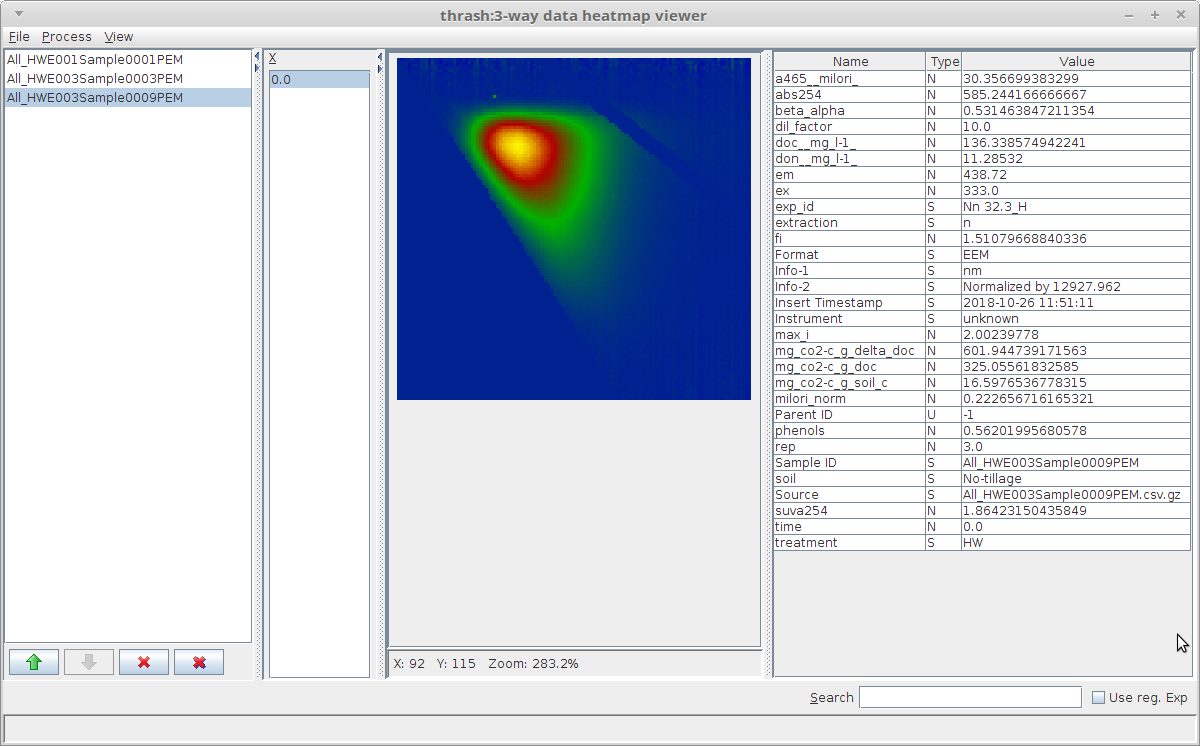
\includegraphics[width=12.0cm]{images/heatmapviewer.png}
  \caption{3-way data heatmap viewer}
  \label{heatmapviewer}
\end{figure}

%%%%%%%%%%%%%%%%%%%%%%%%%%%%%%%%%%%
% Copyright (c) 2009-2012 by the University of Waikato, Hamilton, NZ. 
% This work is made available under the terms of the 
% Creative Commons Attribution-ShareAlike 4.0 license,
% http://creativecommons.org/licenses/by-sa/4.0/.
%
% Version: $Revision: 6032 $

\begin{thebibliography}{999}
  % to make the bibliography appear in the TOC
  \addcontentsline{toc}{chapter}{Bibliography}

  % references
  \bibitem{adams}
    \textit{ADAMS} -- Advanced Data mining and Machine learning System \\
    \url{https://adams.cms.waikato.ac.nz/}{}

  \bibitem{nir}
    \textit{NIR} -- Near-infrared spectroscopy \\
    \url{https://en.wikipedia.org/wiki/Near-infrared_spectroscopy}{}

  \bibitem{mir}
    \textit{MIR} -- Near-infrared spectroscopy \\
    \url{https://en.wikipedia.org/wiki/Mid-infrared}{}

  \bibitem{xrf}
    \textit{XRF} -- X-ray fluorescence \\
    \url{https://en.wikipedia.org/wiki/X-ray_fluorescence}{}

\end{thebibliography}


\end{document}
